\chapter{Opis modelu Social Force}
\label{cha:OpisSocialForce}

Model Social Force \cite{SforceModelForPedDyn}, powszechnie uważany za najważniejszy z obecnie dostępnych modeli symulacji ruchu pieszych \cite{HeBuAjTw}, jest mikroskopowym modelem ciągłym. Zakłada on, że piesi w ruchu mogą zostać w prosty sposób opisani za pomocą sił. Siły te pochodzą nie tylko z oddziaływań konkretnego pieszego na otoczenie, ale także z otoczenia na danego pieszego. Wartość, zwrot oraz kierunek siły finalnej jest składową wszystkich sił działających na danego pieszego. Piesi w modelu reprezentowani są za pomocą cząstek, które dążą do celu w konkretnych kierunkach oraz są pod działaniem wspomnianych sił. Dotychczasowe symulacje komputerowe pokazują, że Model Social Force, pomimo swojej prostoty, bardzo dokładnie oddaje rzeczywiste zachowanie tłumu.

\begin{figure}
\centering
\includegraphics[width=1\textwidth]{process.eps}
\caption{Schemat podejmowania decyzji przez pieszego, opracowanie własne na bazie \cite{GuideCrowdDynViaModifiedSocialForceModel}}
\end{figure}

Nie bez znaczenia jest także łatwość uzyskania parametrów oraz wartości potrzebnych do symulacji. Wartości takie jak predkość $\vec{v_{\alpha}}$ czy położenie $\vec{r_{\alpha}}$ danego pieszego $\alpha$ są łatwe do obliczenia, jak również do skalibrowania z danami empirycznymi.

Pierwotnie SFM wykorzystywany był przede wszystkim w symulacjach ewakuacji budynków. W tego typu sytuacjach celem pieszego jest dojście do wyjścia w możliwie najkrótszym czasie. Obecnie istnieje mnogość wariantów modelu, które pozwalają na zamodelowanie większej ilości zachowań. Modyfikacje przewidują przykładowo unikanie ,,spychania'' innych uczestników ruchu poprzez pieszych poruszających się z większą prędkością \cite{6}, obecność liderów czy panikę.

Wykorzystany w pracy model \cite{GuideCrowdDynViaModifiedSocialForceModel}, bazujący na oryginalnym modelu Helbinga \cite{SforceModelForPedDyn}, zakłada że na pieszego działają trzy siły. Desired force $\vec{f_{i}^{0}}$, siła interakcji pomiędzy pieszymi $i$ oraz $j$, $\vec{f_{ij}}$ oraz siła interakcji pomiędzy pieszym $i$, a przeszkodami, $\vec{f_{iw}}$

Siła działająca na każdego z pieszych definiuje się jako:

\begin{equation}
m_{i} \frac{d\vec{v_{i}}(t)}{dt} = \vec{f_{i}^{0}} + \sum_{j(\neq i)} \vec{f_{ij}} + \sum _{w} \vec{f_{iw}}
\end{equation}

gdzie
\begin{eqwhere}[2cm]
	\item[$m_{i}$] masa pieszego $i$
	\item[$\vec{v}_{i}(t)$] aktualna prędkość
\end{eqwhere}

\section{Desired force}
\label{sec:desiredForce}

Zgodnie z założeniami SFM piesi wykazują niechęć do zmiany prędkości oraz kierunku swojej drogi. Zazwyczaj wybierana jest droga, którą można podążać prosto przez jak najdłuższy okres czasu, nawet jeśli drogi alternatywne są takiej samej długości, a droga wybrana przez pieszego jest mocno zatłoczona. Kierunek ruchu obliczany jest na podstawie wzoru:

\begin{equation}
\vec{e}_{\alpha}(t) = \frac{\vec{r}_{\alpha}^{k} - \vec{r}_{\alpha}(t)}{\parallel \vec{r}_{\alpha}^{k} - \vec{r}_{\alpha}(t) \parallel}
\end{equation}

gdzie
\begin{eqwhere}[2cm]
	\item[$e_{\alpha}(t)$] aktualna pozycja pieszego $\alpha$ w czasie $t$
	\item[$\vec{r}_{\alpha}^{k}$] najbliższy punkt na ścieżce do celu
\end{eqwhere}

\begin{figure}
\centering
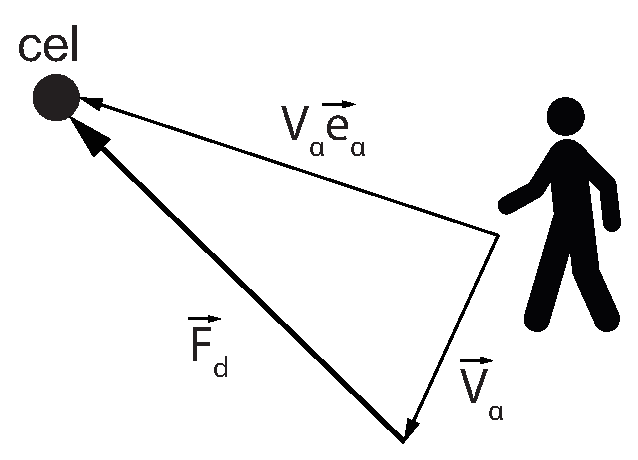
\includegraphics[width=0.5\textwidth]{desiredforce2.eps}
\caption{Schemat siły \textit{desired force} , opracowanie własne na bazie \cite{AMSFMfPBSaSC}}
\end{figure}

\begin{figure}
\centering
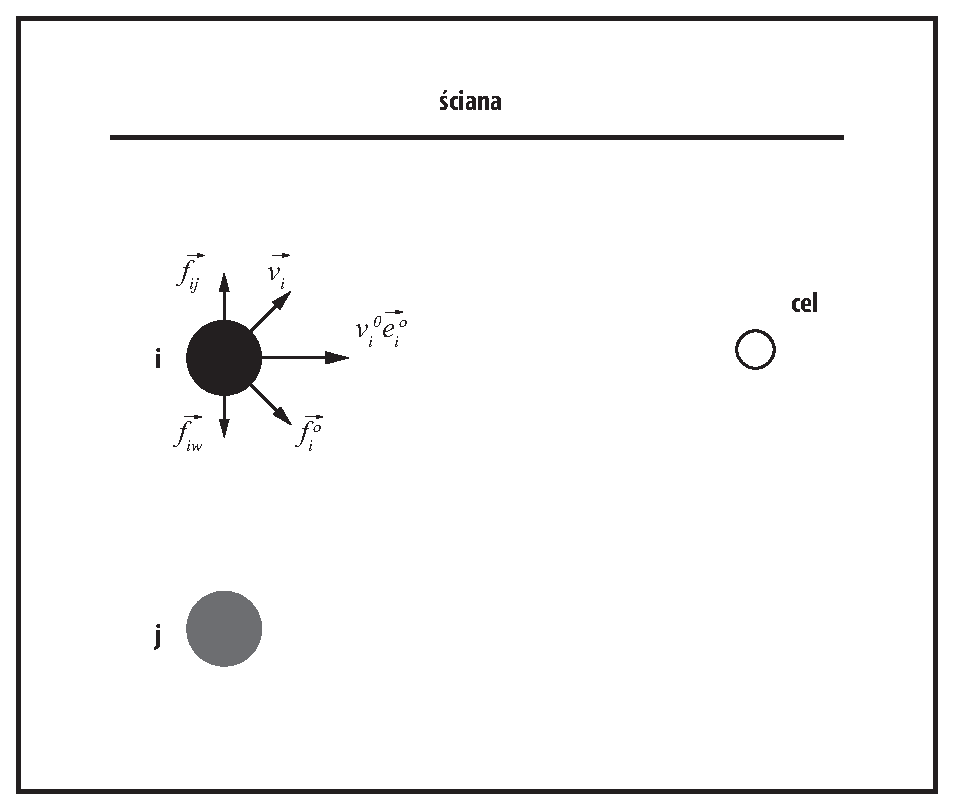
\includegraphics[width=0.7\textwidth]{desiredforce.eps}
\caption{Diagram modelu Social Force, opracowanie własne na bazie \cite{GuideCrowdDynViaModifiedSocialForceModel}}
\end{figure}

W przypadku, kiedy ruch pieszego odbywa się bez przeszkód, porusza się on w kierunku pozycji celu~z preferowaną przez siebie prędkością, $\vec{v_{i}^{0}}$. Z powodu działania na pieszego sił~z otoczenia, obserwuje się dążenie pieszego do osiągnięcia preferowanej przez siebie prędkości w czasie relaksacji $\tau$.

\begin{equation}
\vec{f}_{i}^{0} = m_{i} \frac{v_{i}^{0}(t) \vec{e_{i}^{0}} - \vec{v_{i}}(t)}{\tau}
\end{equation}

gdzie
\begin{eqwhere}[2cm]
	\item[$\vec{v_{i}^{0}}$] wartość domyślnej prędkości pieszego
	\item[$\vec{e_{i}^{0}}$] kierunek ruchu jaki pieszy chce osiągnąć
	\item[$\tau$] czas relaksacji
\end{eqwhere}
	
Jest to tzw. \textit{desired speed} czyli charakterystyczna prędkość dla jednostki, która kierują danego pieszego $i$ do osiągnięcia celu.

Zazwyczaj prędkość pieszego przyjmuje wartość około $1.34 \frac{m}{s}$ \cite{transporttechnikDerFussganger} z odchyleniem standardowym $0.26 \frac{m}{s}$ \cite{HeBuAjTw}.

\section{Interakcja pomiędzy pieszymi}
\label{sec:interactionBetweenPedestrians}

Naturalną reakcją na zbliżanie się do innych uczestników ruchu jest uczucie dyskomfortu. Zakłada się, że każdy z pieszych, który jest w konflikcie z innym uczestnikiem ruchu, generuje wokół siebie eliptyczne pole siły, działające na drugiego z pieszych. Aby uniknąć wypadków, utrzymują oni dystans pomiędzy sobą oraz przeszkodami. Dystans ten zmniejsza się w przypadku pośpiechu pieszego oraz wzrastu gęstość tłumu. Gęstość tłumu zwiększa się w szczególności, kiedy piesi znajdują się w okolicy miejsc wzbudzających większe zainteresowanie oraz w wąskich przejściach (tzw. wąskie gardła). Siła interakcji pomiędzy pieszymi $i$ oraz $j$, $\vec{f_{ij}}$ definiowana jest jako suma dwóch sił (wzór \ref{eq:sumaSil}), socjologiczno-psychologicznej oraz fizycznej. Piesi mogą także formować grupy, których zachowanie można później sprowadzić do opisu pojedynczego agenta \cite{HeBuAjTw}

\begin{equation}
\label{eq:sumaSil}
\vec{f_{ij}} = \vec{f}_{ij}^{s} + \vec{f}_{ij}^{p}
\end{equation}
Pierwsza z nich $\vec{f_{ij}^{s}}$ (wzór \ref{eq:socioSila}) związana jest z naturalnym ludzkim odruchem utrzymywania odpowiednich odległości pomiędzy osobami w poruszającej się grupie ludzi. Przyjmuje ona wartość maksymalną, gdy odległość między dwoma pieszymi $d_{ij}$ maleje, a wartość mniejszą w przypadku oddalania się pieszych.

\begin{equation}
\label{eq:socioSila}
\vec{f_{ij}^{s}} = A_{i} exp[(r_{ij} - d_{ij}) / B_{i}]\vec{n_{ij}}
\end{equation}

gdzie
\begin{eqwhere}[2cm]
	\item[$A_{i}$] intensywność działania siły
	\item[$B_{i}$] Dystans działania siły
	\item[$\vec{n_{ij}}$] wektor jednostkowy o początku w centrum strefy prywatnej pieszego $i$ a końcu~w centrum tej strefy pieszego $j$
\end{eqwhere}

Druga z sił $\vec{f_{ij}^{p}}$ (wzór \ref{eq:silaFizyczna}) oddziałuje na pieszych, kiedy dystans pomiędzy dwoma pieszymi, $d_{ij}$ jest mniejszy od sumy promieni ich stref prywatnych $r_{ij} = r_{i} + r_{j}$. Siła ta składa się z \textit{body force}, $\vec{f} _{ij}^{p_{1}}$ oraz \textit{sliding friction force}, $\vec{f} _{ij}^{p_{2}}$.

\begin{equation} \label{eq:silaFizyczna}
\vec{f}_{ij}^{p} = kg(r_{ij} - d_{ij})\vec{n}_{ij} + \kappag (r_{ij} - d_{ij}) \Delta v_{ij}^{t}\vec{t}_{ij}
\end{equation}

gdzie
\begin{eqwhere}[2cm]
	\item[$k$] body compression coefficient
	\item[$\kappa$] Coeficient of sliding friction
	\item[$\vec{n}_{ij}$] wektor jednostkowy o początku w pozycji pieszego $i$ a końcu w pozycji pieszego $j$
	\item[$\Delta v_{ij}^{t} \cdot \vec{t}_{ij}$] zmiana prędkości wzdłuż stycznej do eliptycznego pola strefy prywatnej
\end{eqwhere}

\begin{equation}
g(x) = \left\{ 
\begin{array}{c l}	
     0, & dla x < 0,\\
     x, & dla x \geq 0.
\end{array}\right.
\end{equation}

Warto zaznaczyć, że druga z sił przyjmuje pewne wartości nawet w przypadku, kiedy dwoje pieszych znajduje się daleko od siebie. Oznacza to, że piesi zawsze starają się utrzymać między sobą dystans \cite{relativeVelocity}.


\section{Zalety i wady Modelu Social Force}

Największą z zalet opisywanego modelu jest precyzja odwzorowania zachowań mikroskopowych oddziaływań pomiędzy pieszymi oraz otaczającą ich rzeczywistością. SFM uwzględnia wiele powszechnych tendencji, takich jak:

\begin{itemize}
\item Unikanie kontaktu z przeszkodami oraz innymi uczestnikami ruchu przed dojściem do kolizji,
\item \textit{Szybciej znaczy wolniej}, wraz ze wzrostem prędkości jednostek, rożnie zatłoczenie miejsc, w których się poruszają (takich jak obszary wokół wyjścia z budynków), co skutkuje spowolnieniem ruchu,
\item formowanie strug, czyli skłonność pieszych do poruszania się w liniach. Zachowanie to może być zauważone w szczególności, kiedy dwie grupy ludzi poruszają się w przeciwnych kierunkach.
\end{itemize}
Pomimo licznych zalet, model nie jest pozbawiony wad. Pierwszą z nich jest mała wydajność obliczeniowa oraz trudności z odwzorowaniem niektórych sytuacji. Mnogość sił, które są obliczane, w przemnożeniu poprzez ilość pieszych powoduje wysoki narzut na ilość obliczeń. W~tym miejscu dużą konkurencją stają się automaty komórkowe, które nie wymagają tak skomplikowanych obliczeń, dając jednocześnie szerokie spektrum odwzorowania zróżnicowanych zachowań ruchu pieszych. Drugą z wad są oscylacje w jakie wpada pieszy, kiedy brakuje mu swobody przemieszczania.
